% !TeX program = xelatex
\documentclass[11pt,a4paper]{article}

\usepackage{fontspec}
\setmainfont{Libertinus Serif}
\usepackage{polyglossia}
\setdefaultlanguage{serbian}
\setotherlanguage{english}
\usepackage{geometry}
\usepackage{graphicx}
\usepackage{xcolor}
\usepackage{enumitem}
\usepackage{hyperref}
\usepackage{bookmark}
\usepackage{microtype}
\usepackage{parskip}
\usepackage{fvextra}
\usepackage{float}
\usepackage{caption}

\geometry{margin=2.2cm}
\setlength{\emergencystretch}{3em}
\setlist{leftmargin=*}
\urlstyle{same}
\hypersetup{
  colorlinks=true,
  linkcolor=blue!50!black,
  urlcolor=blue!50!black,
  pdfcreator={LaTeX via pandoc}
}
\providecommand{\tightlist}{%%
  \setlength{\itemsep}{0pt}\setlength{\parskip}{0pt}}
\DefineVerbatimEnvironment{CodeBlock}{Verbatim}{breaklines=true,breakanywhere=true,fontsize=\small}

\title{Git}
\date{}

\begin{document}
\maketitle

\section{Šta je git objašnjeno na jednostavnom
primjeru}

Jedna od brojnih mogućnosti koje ti git nudi jeste istorija izmjena.
Zamisli neki editor, bilo koji. Svaki editor ima ugrađenu mogućnost
``\emph{undo} pomoću koje možeš da poništiš prethodnu akciju. Većina
editora ti omogućuju da poništiš i više prethodnih akcija i vratiš se u
prošlost. Git ti nudi istu stvar ali u kodu. Razlika između git-a i
editora je to što editor za tebe pamti akcije koje su se desile, a git
ne pamti, već ti sam praviš svoje verzije. Verzija bi bila neko stanje
projekta koje želiš da sačuvaš u istoriji, na koje se možda želiš
vratiti u budućnosti.

Druga bitna stvar vezana za git je praćene sadržaja. Rekli smo iznad da
git za tebe ne pamti akcije koje su se desile. Međutim, git zato prati
sadržaj i prikazuje ti sve promjene koje su se desile. Npr. u editoru si
dodao novu liniju koda u jedom fajlu, dodao si 10 linija u drugom i
napravio novi fajl. Git će ti prikazati sve ove izmjene, gdje ti onda od
ovih izmjena možeš napraviti novu verziju. Novu verziju ne moraš praviti
od svih izmjena, možeš da odabereš neki podskup. Kad praviš novu verziju
potrebno je da opišeš zašto si napravio te izmjene, kako bi kasnije kad
bi se htio vratiti na nju lako mogao naći koja ti verzija treba.

\emph{Napomena:} Ovo objašnjenje, ali i samo uputstvo, je veoma
pojednostavljeno. Git ima dosta više mogućnosti od ovdje navedenih.
Naredbe i komande su objašnjene tek toliko koliko ti je potrebno da
kreneš sa radom. Git ima odličnu dokumentaciju koja će biti linkovana na
svim mjestima. Toplo preporučujem literaturu koja je navedena pri kraju
dokumenta. Ideja ovog dokumenta je da te uvede u priču o gitu, a kasnije
ćeš sam širiti svoje znanje i git mastery.

\section{Uvod}

Git je distribuirani sistem za kontrolu verzija. Prednosti:

\begin{itemize}
\item
  brz i skalabilan
\item
  jednostavan dizajn
\item
  odlična podrška za paralelan rad
\item
  ne prati fajlove već sadržaj
\end{itemize}

Git istoriju modeluje pomoću usmjerenog acikličnog grafa sa promjenama.
Možemo se kretati kroz graf, širiti ga, granati, itd. Svaki čvor u grafu
predstavlja jedan commit.

Da za početak pojednostavimo priču, commit možeš posmatrati kao jednu
verziju tvog projekta. Git je napravljen tako da kad se krećeš između
commit-ova izgleda kao da se krećeš između verzija tvog projekta. Ipak,
ispod haube ovo nije tako. U paragrafu ispod imaš kratko objašnjenje
kako on zapravo radi.

\emph{Za one koji žele da znaju više}: Commit predstavlja samo skup
izmjena. Da bi dobio verziju tvog projekta u nekom commit-u, potrebno je
da se primjene svi commit-i (svi skupovi izmjena) od prvog (inicijalnog
commit-a koji predstavlja početno stanje tvog projekta) do trenutnog
commit-a i tek tada dobiješ trenutno stanje.

\begin{center}
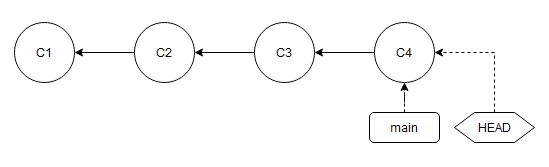
\includegraphics[width=5.71955in,height=1.73983in,alt={Diagram Description automatically generated}]{assets/media/image1.png}
\end{center}

Slika 1. Primjer jednog git grafa

Na slici iznad su krugovima sa oznakama C1, C2, C3 i C4 označeni
commit-ovi. Commit predstavlja skup izmjena. C1 je inicijalni commit i
on predstavlja početno stanje projekta. Svaki commit ima referencu na
svog prethodnika i tako dobijemo graf. Grane su na slici označene sa
pravougaonicima sa zaobljenim ivicama i unutar njih su imena grana. Na
slici trenutno ima samo jedna grana main. Pored commit-a i grana na
slici možemo uočiti i HEAD koji se nalazi u dijamantu. HEAD nam govori
gdje se trenutno nalazimo unutar grafa (u ovom slučaju nalazimo se na
commit-u C4 na grani main).

Spomenuli smo grane, pa je red i da ih kratko objasnimo. Grane su tokovi
razvoja. Možeš ih pojednostavljeno posmatrati kao zasebne kopije tvog
projekta. Kad radiš na jednoj grani, ostale kopije (grane) su netaknute.
Možeš lako da se prebaciš sa jedne grane na drugu i počneš razvoj nove
funkcionalnosti, itd.

Mogućnosti grana se najbolje ogledaju u timskom radu. \textbf{Uz pomoć
grana} \textbf{svi članovi tima mogu zajedno da rade na istom projektu u
isto vrijeme}. Ovo je jedna od velikih prednosti korišćenja gita. Grane
ti omogućuju da paralelno radiš na projektu sa tvojim članovima tima,
možeš da šalješ svoje grane (posao koji si odradio) drugim članovima
tima, oni mogu da nastave rad gdje si stao. Po vrh svega, možeš da
spajaš grane i tako integrišeš posao koji je razvijan paralelno u jednu
granu koja će onda sadržati sve izmjene.

\section{Instalacija}

Git možeš preuzeti na: \url{https://git-scm.com/downloads}

Instalacija je prilično jednostavna, savjet je da pažljivo pratiš korake
instalacije jer tu biraš podrazumijevani editor za rad sa git-om.
Inicijalna vrijednost je Vim i preporuka je da odabereš neki drugi
ukoliko nisi upoznati sa Vim-om. Nije problem ukoliko odabereš pogrešan
editor, lako ga možeš zamijeniti kasnije
(\href{https://stackoverflow.com/questions/2596805/how-do-i-make-git-use-the-editor-of-my-choice-for-commits}{uputstvo}).

\section{Konfiguracija}

Git je veoma konfigurabilan. Konfiguracija se može podesiti na globalnom
nivou, na nivou korisnika i na nivou projekta. Tako možeš imati
različita podešavanja kad radiš na različitim projektima. Za detalje
pogledaj \url{https://git-scm.com/docs/git-config}.

Par stvari je potrebno da odmah konfigurišeš: (Ukoliko radiš u učionici
u kojoj više studenata dijeli isti laptop, ne preporučujem da radiš ovo
podešavanje sad, već nakon što napraviš novi git repozitorijum pokreni
ovu komandu unutar njega (repozitorijuma) bez flag-a --global. Ovako će
tvoje ime i email biti podešeni samo za taj tvoj projekat, a ne za
cijeli sistem.)

\begin{itemize}
\item
  ime korisnika: git config -\/-global user.name "Marko Marković"
\item
  email korisnika: git config -\/-global user.email marko@example.com
\end{itemize}

Ime i email koje se ovdje definišu će se koristiti kao ime i email
autora commit-ova. Konfiguraciju možeš izlistati sa git config -\/-list.

\section{Praćenje sadržaja}

Git radi tako što prati promjene svih fajlova unutar repozitorijuma
(\emph{radnog stabla}). Ukoliko želimo da git ignoriše neke fajlove
potrebno je da napravimo .gitignore fajl
\url{https://git-scm.com/docs/gitignore}.

Kad smo odabrali izmjene koje želimo da spremimo za commit prebacujemo
ih u \emph{pripremnu zonu} (\emph{index}).

Kad su svi fajlovi koji idu u commit u \emph{index}-u sa \emph{commit}
naredbom pravimo novi commit od fajlova iz \emph{index}-a i smještamo ih
u \emph{lokalni repozitorijum}. Ovaj workflow je ilustrativan na slici
ispod. Na ovaj način možemo samo dijelove koda da komitujemo i biramo
šta od promjena ide u lokalni repozitorijum.

\begin{center}
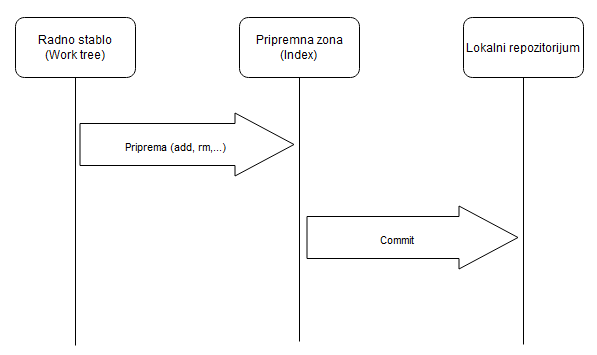
\includegraphics[width=6.16275in,height=3.66462in,alt={Diagram Description automatically generated}]{assets/media/image2.png}
\end{center}

Slika 2. Radno stablo -- pripremna zona -- lokalni repozitorijum

\section{Praktičan primjer}

Sad ćemo na primjeru vrlo jednostavnog kalkulatora objasniti rad sa
git-om. Kalkulator prima kao unos string koji je u formatu: "broj
operacija broj", zatim parsira string, izvrši operaciju i korisniku
ispisuje rezultat. Ukoliko korisnik kao unos proslijedi "kraj" ili
"exit" aplikacija se gasi.

\begin{itemize}
\item
  U svom editoru generiši i otvori novi projekat
\item
  Pokreni git bash (ukoliko si na Windows-u) ili bilo koji terminal
  emulator (ukoliko si na nekom od Unix derivata) i pozicioniraj se u
  direktorijum u kom se nalazi tvoj projekat
\item
  Inicijalizuj git repozitorijum

  \begin{itemize}
  \item
    git init - inicijalizuje git repozitorijum unutar trenutnog foldera
  \end{itemize}
\item
  Provjeri stanje repozitorijuma git status prikaže trenutno stanje,
  koje uključuje:

  \begin{itemize}
  \item
    promjene nad fajlovima koje git prati
  \item
    promjene nad fajlovima koje git ne prati
  \end{itemize}
\end{itemize}

Možeš uočiti da su se pojavili fajlovi iz projekta, za koje git kaže da
ih trenutno ne prati.

Inicijalno git ne prati sadržaj fajlova dok ih prvi put ne dodamo u
index, nakon toga on kreće sa praćenjem izmjena.

\subsection{Ignorisanje fajlova}

Nekad ne želimo da git prati sve fajlove ili foldere iz repozitorijuma.
Tu nam u pomoć uskače .gitignore fajl. U ovaj fajl je potrebno da
navedemo putanje do fajlova ili foldera koje želimo da git ignoriše.
Više o ovom fajlu i ignorisanju možeš naći na zvaničnoj
\href{https://git-scm.com/docs/gitignore}{dokumentaciji}. Neke početne
.gitignore fajlove možeš naći na idućem
\href{https://github.com/github/gitignore}{repozitorijumu}. Druga opcija
je da generišeš ovaj fajl. Možeš koristiti
\href{https://www.toptal.com/developers/gitignore}{ovaj sajt}. Potrebno
je da navedeš IDE ili editor koji koristiš za razvoj i programske jezike
koje koristiš (npr. za c\# možete navesti: Rider, Visual Studio, Visual
Studio Code, Csharp) . Nakon toga se generiše fajl koji možeš smjestiti
u korijen repozitorijuma. Nakon što dodaš .gitignore sve što si naveo u
njemu će biti ignorisano i više se neće pojavljivati u statusu.

\subsection{Dodavanje i uklanjanje izmjena u
index}

Dalje, želimo da dodamo projektne fajlove u index da bi napravili prvi
commit. U nastavku su pobrojane najbitnije naredbe za prebacivanje
izmjena između index-a i radnog stabla. \emph{Tip}: dok analiziraš ove
naredbe, posmatraj sliku 2 i vizualizuj šta tačno radi svaka od ovih
naredbi.

\begin{itemize}
\item
  git add .- dodaće sve fajlove iz trenutnog direktorijuma i svih
  poddirektorijuma rekurzivno u index zonu. Umjesto tačke možeš navesti
  ime jednog fajla, ili više fajlova razdvojenih razmakom.
\item
  git add \textless putanja do fajla\textgreater{} - dodaje navedeni
  fajl u index. Moguće je dodati više fajlova, gdje se onda navodi
  putanja do svakog fajla. Putanje se razdvajaju razmakom.
\item
  git rm -- uklanja fajl iz index-a i iz radnog stabla (koristi flag
  -\/-cached da bi fajl uklonio samo iz index-a)
\item
  git restore -\/-staged -- vraća fajl iz index-a u radno stablo (ostaju
  sve promjene u fajlu, samo više neće biti u index-u).

  Sa git add . prebaci sve fajlove u index.
\end{itemize}

\subsection{Pravljenje commit-a}

Kada se fajlovi nalaze u index-u, možemo da napravimo prvi commit:

\begin{itemize}
\item
  git commit - otvara editor za unos commit poruke. U komentarima ispod
  je izlistano šta će biti komitovano, a šta ostaje u index-u (ovdje
  možete provjeriti da li ste odabrali sve što ste željeli).
\item
  Za commit poruku možete unijeti "Initial commit". Imajte u vidu da
  pišete \href{https://chris.beams.io/posts/git-commit/}{kvalitetne
  commit poruke}. Commit poruke pišite na engleskom.
\end{itemize}

\subsection{Istorija}

Možemo provjeriti graf promjena našeg repozitorijuma sa:

\begin{itemize}
\item
  git log - prikaže istoriju commit-ova sa informacijama o svakom od
  njih.
\end{itemize}

Možemo uočiti da ima samo jedan commit koji smo upravo napravili i mi
smo autor tog commit-a.

\begin{itemize}
\item
  gitk -- grafički alat pomoću kog možemo da pregledamo istoriju
\end{itemize}

Vraćamo se u editor i razvijamo novu funkcionalnost za naš mini
projekat. Potrebno je da omogućimo korisniku da unese neki tekst. Učitaj
od korisnika proizvoljan tekst i ispiši ga.

Nakon što si se uvjerio da funkcionalnost radi, vrati se u git bash i
ponovi korake od ranije: git status da vidiš izmjene, zatim sa git add
\textless fajl\textgreater{} dodaj fajlove koje želiš da commit-uješ i
sa git commit napravi commit i unesi smislenu poruku. Uvjeri se da je
sve u redu sa git log i opciono provjeri stanje repozitorijuma git
status.

Idući korak je da dodaš petlju u kojoj će kalkulator primati naredbe.
Ukoliko korisnik unese exit petlja se završava. Commit-uj.

Proširi prethodnu petlju tako da se petlja završi ukoliko korisnik unese
exit ili kraj. Commit-uj.

Implementiraj parsiranje stringova po razmaku i validiraj da ima tačno 3
ulazna parametra. Commit-uj.

Ako pogledaš log u obliku grafa, trebao bi dobiti nešto slično kao na
slici ispod:

\begin{center}
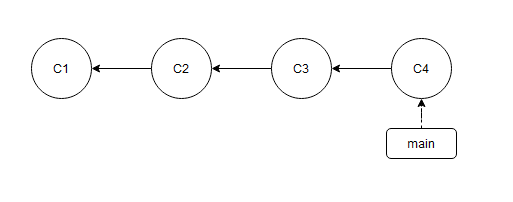
\includegraphics[width=5.18375in,height=2.04116in,alt={Diagram Description automatically generated}]{assets/media/image3.png}
\end{center}

Isprobaj komandu git checkout pomoću koje se možemo kretati git grafom.
Ova komanda kao parametar prima hash commit-a i prebacuje se na njega.
Prebaci se na neki od ranijih commit-ova i pogledaj šta se dešava sa
projektom u tvom editoru.

\section{Grane}

Pravimo kraku pauzu od projekta da bi se osvrnuli na koncept grana u
gitu. Grana predstavlja alternativni tok razvoja. To znači da paralelno
možemo raditi na dvije (ili više) funkcionalnosti bez ikakvih problema i
kad smo završili samo spojimo (engl. \emph{merge}) izmjene na glavnu
granu razvoja. Pored ovoga, grane su zgodne jer možemo da isprobamo neku
implementaciju i ako ne radi lako odustanemo od nje tako što izbrišemo
granu, a izvorni kod aplikacije ostaje netaknut na glavnoj grani.

\begin{center}
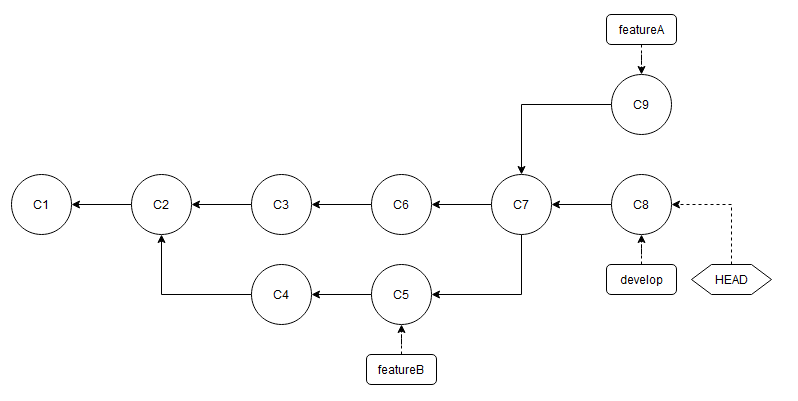
\includegraphics[width=5.592in,height=2.80963in,alt={Diagram, schematic Description automatically generated}]{assets/media/image4.png}
\end{center}

Na slici iznad je prikazan proširen graf sa više grana. Sad vidimo da
više commit-ova može imati istog roditelja (C3 i C4 imaju roditelja C2).
Ovo su alternativni tokovi razvoja -- grane. Grane su prikazane u
pravougaonicima sa zaobljenim ivicama. Pored toga, jedan commit može
imati i dva roditelja (C7 ima roditelje C5 i C6). Ovaj commit se naziva
\emph{merge-commit} i predstavlja spajanje grana. Spajanje grana
integriše izmjene sa jedne grane na drugu.W

\subsection{Pravljenje grana i prelazak na
granu}

Vraćamo se projektu:

\begin{itemize}
\item
  započećemo razvoj nove funkcionalnosti na novoj grani:
\item
  git branch feature/addition će napraviti novu granu sa nazivom
  feature/addition
\item
  da bi se prebacili na granu koju smo upravo kreirali koristimo komandu
  git checkout feature/addition

  U git bash-u ili terminal emulatoru, možete primjetiti da je naziv
  grane promijenjen i u samom emulatoru. Izvrši git log naredbu i vidi
  kako trenutno izgleda git graf.
\end{itemize}

\begin{center}
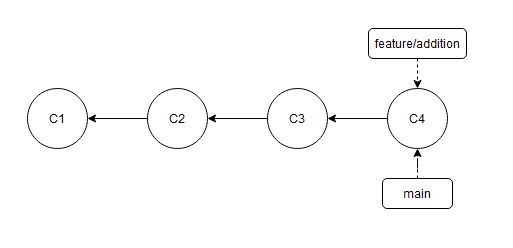
\includegraphics[width=3.6623in,height=1.77047in,alt={Diagram Description automatically generated}]{assets/media/image5.png}
\end{center}

Na novoj grani parsiraj stringove u brojeve, uvjeri se da sve radi uredu
i commit-uj.

Dodaj funkciju za sabiranje brojeva i integriši je unutar glavne petlje.
Uvjeri se da radi kako treba i commit-uj.

\begin{center}
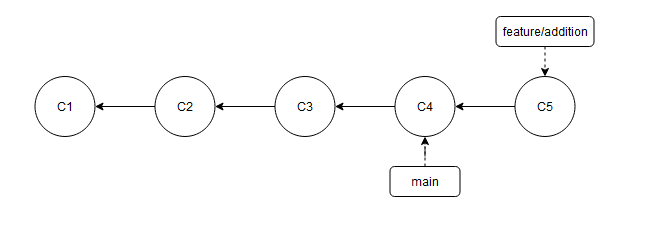
\includegraphics[width=4.51955in,height=1.64889in,alt={Diagram Description automatically generated}]{assets/media/image6.png}
\end{center}

\subsection{Spajanje grana}

Kad smo završili sa razvojem i želimo da novu funkcionalnost integrišemo
u glavnu granu radimo \emph{merge}:

\begin{itemize}
\item
  Da bismo spojili feature/addition granu na našu glavnu granu (što je
  kod nas main) prvo je potrebno da se prebacimo na main granu. Prebaci
  se na main granu (obrati pažnju na editor i sadržaj projekta nakon što
  si se prebacio).
\item
  Sa git merge feature/addition git spaja feature/addition granu sa
  main. Pogledaj git log i prodiskutuj sa asistentom rezultate.

  \begin{center}
  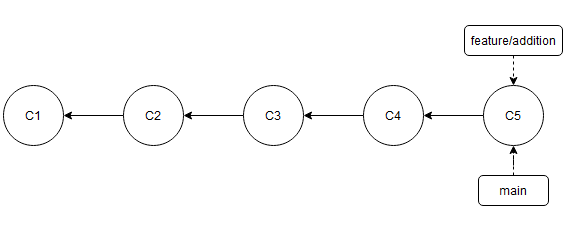
\includegraphics[width=5.01023in,height=1.968in,alt={Diagram Description automatically generated}]{assets/media/image7.png}
  \end{center}

  Na sličan način implementiraj oduzimanje na grani
  feature/substraction, provjeri da li radi, commit-uj i spoji.

  \begin{center}
  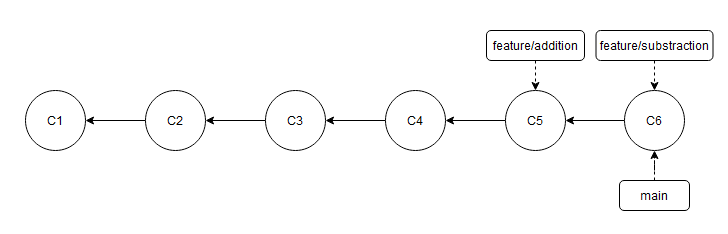
\includegraphics[width=4.91422in,height=1.57945in,alt={Diagram Description automatically generated}]{assets/media/image8.png}
  \end{center}
\item
  Izvrši git log ili pokreni git-ov integrisani alat za grafički prikaz
  grafa repozitorijuma gitk. Analiziraj sa asistentom alat.

  Opciono: poigraj se sa komandama git show i git diff. Pročitaj
  dokumentaciju i primjeni ih na repozitorijum.
\end{itemize}

\section{Konflikti}

Ponekad se desi da se u toku razvoja moraju mijenjati isti fajlovi i čak
iste linije unutar fajlova. Pitanje je kako održati konzistentno stanje
repozitorijuma ako se na dvije grane paralelno izmjeni ista linija koda.
Git sam može da riješi spajanje ukoliko su različite linije izmjenjene,
ali ako je ista linija ili iste linije promijenjena na dvije grane
potrebno je da mu pomognemo da razriješi taj problem. Ova pojava u git-u
se naziva merge conflict i tad git staje sa merge naredbom i prepušta
nama da riješimo konflikte i dovršimo merge.

Vratimo se projektu i hajde da vještački izazovemo jedan konflikt tako
što ćemo na main grani razviti jednu funkciju koja množi brojeve, a na
grani feature/division implementirati funkciju koja dijeli brojeve i
uvezati je sa ostatkom projekta.

\begin{itemize}
\item
  Prebaci se na main granu, ako već nisi na njoj.
\item
  Napravi novu granu feature/division i prebaci se na nju, na toj grani
  implementiraj funkciju za dijeljenje brojeva, commit-uj.
\item
  Vrati se na main granu
\item
  Napravi funkciju koja množi brojeve, commit-uj izmjene. Obrati pažnju
  da se barem jedna linija koda ove funkcije poklapa sa funkcijom na
  feature/division grani.
\item
  Spoji feature/division na main.
\end{itemize}

Prodiskutuj sa asistentom rezultat ovog pokušaja merge-a.

\begin{center}
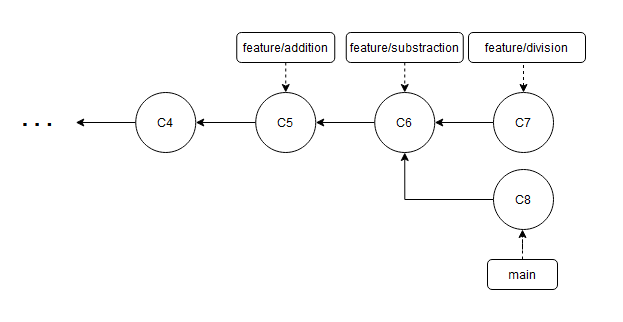
\includegraphics[width=4.03993in,height=2.088in,alt={Diagram Description automatically generated}]{assets/media/image9.png}
\end{center}

\subsection{Razrješavanje
konflikata}

Dakle konflikti nastanu kad paralelno izmijenimo iste linije koda, pa
git nije siguran kako da izvrši merge. Git onda svaki od konflikata
označi markerima koji izgledaju ovako:

\textless\textless\textless\textless\textless\textless\textless{}
HEAD:file

..... (u ovom prvom dijelu se nalazi trenutna izmjena - to su izmjene na
grani na kojoj smo bili kad smo započeli merge)

=======

..... (u drugom dijelu su izmjene na drugoj grani - granu koju smo
htjeli da merge-ujemo)

\textgreater\textgreater\textgreater\textgreater\textgreater\textgreater\textgreater{}
\textless naziv grane ili commit-a\textgreater:file

~

Potrebno je da svaki od konflikata riješiš, dodaš promjene koje si
napravio da bi riješio konflikte u index zonu i komituješ. Ovdje će ti
se sama commit poruka popuniti koju možeš zadržati.

Primjer konflikta:

\begin{enumerate}
\def\labelenumi{\arabic{enumi}.}
\item
  \textless\textless\textless\textless\textless\textless\textless{}
\item
  private double Multiply(double a, double b) \{
\item
  return a*b;
\item
  \}
\item
  =======
\item
  private double Divide(double a, double b) \{
\item
  return a/b;
\item
  \}
\item
  \textgreater\textgreater\textgreater\textgreater\textgreater\textgreater\textgreater{}
\item
  ~
\end{enumerate}

Sličan konflikt bi trebao imati i ti ako si pratio korake iznad. Da bi
riješio konflikt treba da odlučiš šta nam od ovih promjena treba. U ovom
slučaju želimo da zadržimo obje funkcije, pa prvo ukloni markere
("\textless\textless\textless\textless", "====",
"\textgreater\textgreater\textgreater\textgreater") i provjeri da li sve
radi kako treba. Ukoliko je sve u redu, dodaj izmjene u index zonu i
commit-uj. Nakon commit-a provjeri kako izgleda graf i prodiskutuj
stanje grafa sa asistentom.

\begin{center}
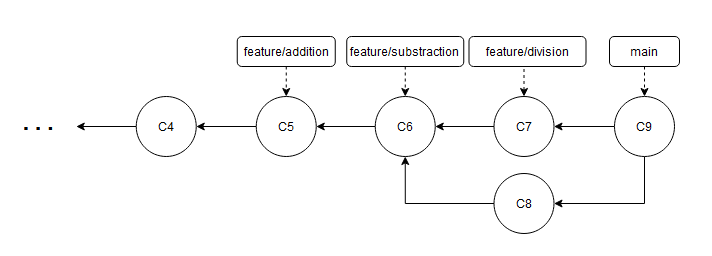
\includegraphics[width=5.71879in,height=2.056in,alt={Diagram Description automatically generated}]{assets/media/image10.png}
\end{center}

Vraćamo se na projekat, sad treba da imaš sve izmjene na main grani.
Vođa tima je odlučio da se od sad na main commit-uju samo nova izdanja
projekta. Napravi develop granu od main grane na kojoj ćeš da razvijaš
ostatak projekta.

\begin{itemize}
\item
  Implementiraj na feature grani funkcionalnost računanja eksponenta u
  obliku: x \^{} y. Na drugoj feature grani implementiraj funkciju koja
  ispisuje "Hello, friend!". Spoji prvu feature granu u develop. Spoji
  drugu feature granu u develop i usput riješi konflikte
\item
  Na novoj feature grani dodaj podršku za sabiranje stringova. Ukoliko
  je korisnik unio dva stringa, kao rezultat sabiranja ispiši
  konkatenovan string.
\item
  Vrati se na develop i napravi novu feature granu koja dodaje podršku
  za množenje stringova. Ukoliko je jedan parametar unosa string (neka
  to bude x), a drugi broj (recimo y), kao rezultat ispiši y puta
  ponovljen string x (primjer: za ulaz a * 3 ispiši aaa).
\item
  Spoji obje feature grane i riješi konflikte usput.
\item
  Spoji develop na main.
\item
  Napravi novu feature granu, na njoj implementiraj istoriju
  kalkulatora. Kad god se unese nova naredba, potrebno je da je sačuvaš
  u fajl pod nazivom \emph{history.txt}. Nemoj da commit-uješ
  \emph{history.txt} fajl. Nakon što si commit-ovao logiku
  implementacije istorije, u .\emph{gitignore} dodaj \emph{history.txt}
  fajl i commit-uj.
\end{itemize}

Na kraju bi tvoj repozitorijum trebao imati strukturu kao na slici
ispod.

\begin{center}
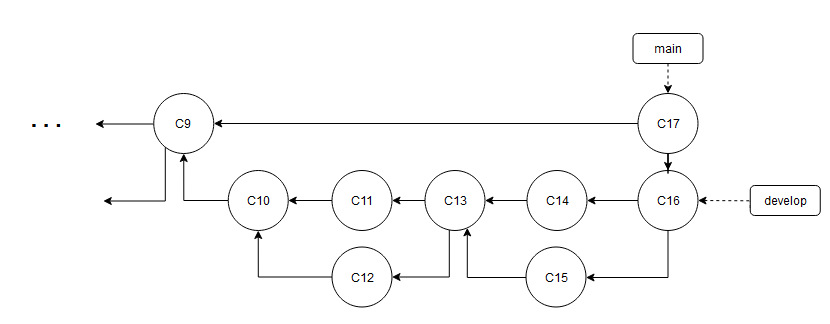
\includegraphics[width=6.18984in,height=2.416in,alt={Diagram, schematic Description automatically generated}]{assets/media/image11.png}
\end{center}

\section{Udaljeni repozitorijumi i udaljene
grane}

Kad smo naučili kako da radimo sa gitom u lokalu, vrijeme je da naučimo
kako možemo da razmjenjujemo izmjene sa kolegama. Pored lokalnih grana
postoje i udaljene grane. Udaljene grane se nalaze na udaljenim
repozitorijumima. Za lokalni repozitorijum možete podesiti više
udaljenih repozitorijuma i slati i dobavljati izmjene sa njih. Obično
bude jedan udaljeni repozitorijum koji se obično zove origin. Da bi
podesili udaljeni repozitorijum za vaš lokalni repozitorijum izvršite
naredbu: git remote add origin \textless url do udaljenog
repozitorijuma\textgreater. Praksa je da se glavni udaljeni
repozitorijum zove origin. Za link do udaljenog repozitorijuma stavite
link do praznog \emph{GitLab/GitHub} repozitorijuma koji ste napravili
ranije.

Da biste provjerili koji udaljeni repozitorijumi su dodati izvršite: git
remote -v. Prodiskutuj sa asistentom rezultat izvršavanja ove naredbe.

\subsection{Slanje izmjena}

Kad smo podesili udaljeni repozitorijum, vrijeme je da na njega
pošaljemo sve što smo razvili u lokalu. Da bi to odradili koristimo
komandu push. Ova komanda šalje sve izmjene sa lokalne grane na udaljenu
granu. Šalju se samo nove izmjene koje ne postoje na udaljenoj grani.
\textbf{Da bi izvršili komandu potrebno je da kažemo gitu na koji
udaljeni repozitorijum šaljemo izmjene i na koju granu tog
repozitorijuma}. Pošalji izmjene na udaljeni repozitorijum koji si
ranije kreirao sa: git push origin \textless ime udaljene
grane\textgreater. Obično ime udaljene grane odgovara imenu lokalne
grane, mada to ne mora da bude slučaj. Ukoliko ime grane ne postoji na
udaljenom repozitorijum, nova grana sa tim imenom će biti kreirana. Da
ne bi svaki put kucao ime udaljenog repozitorijuma i udaljene grane
možeš podesiti podrazumijevanu udaljenu granu na koju će se slati
izmjene sa tvoje lokalne grane. To radiš sa git push -u origin
\textless ime udaljene grane\textgreater. Kad ovo podesiš, svaki idući
put možeš da šalješ izmjene samo sa git push.

\subsection{Dobavljanje izmjena}

Da bi dobavio izmjene sa udaljenog repozitorijuma koristimo naredbu git
fetch origin. Ova naredba dovuče sve nove izmjene sa udaljenog
repozitorijuma. Te izmjene su smještene u takozvanim remote tracking
granama (granama koje prate udaljene grane). Remote tracking grane su
oblika remotes/origin/\textless ime grane\textgreater{} i one su
\emph{read-only} (samo su za čitanje, ne mogu se slati izmjene na njih).
Na remote tracking grane se dovuku izmjene sa udaljenih grana. Da bi te
izmjene integrisali sa našim lokalnim granama radimo git merge
origin/\textless ime grane\textgreater, isto kao kada spajamo dvije
lokalne grane. Kako konflikti nastaju prilikom spajanja lokalnih grana,
isto tako mogu nastati prilikom dobavljanja izmjena sa udaljene grane.

Kako se uvijek radi git fetch origin, pa git merge origin/\textless ime
grane\textgreater, git ima skraćenicu za to: git pull origin
\textless ime grane\textgreater. Savjet je da na početku rada koristiš
\emph{fetch/merge} kombinaciju, dok se ne navikneš na tok rada, pa sa
vremenom pređeš na pull zbog brzine. Slično kao i kod push komande, ako
se podesi default-na push/pull grana, naredba se može pozivati samo sa
git pull.

Na slici ispod su prikazani tipovi grana u gitu i komande koje koristimo
da upravljamo njima. Detaljno analiziraj sliku sa asistentom i
prodiskutujte sve vrste grana.

\begin{center}
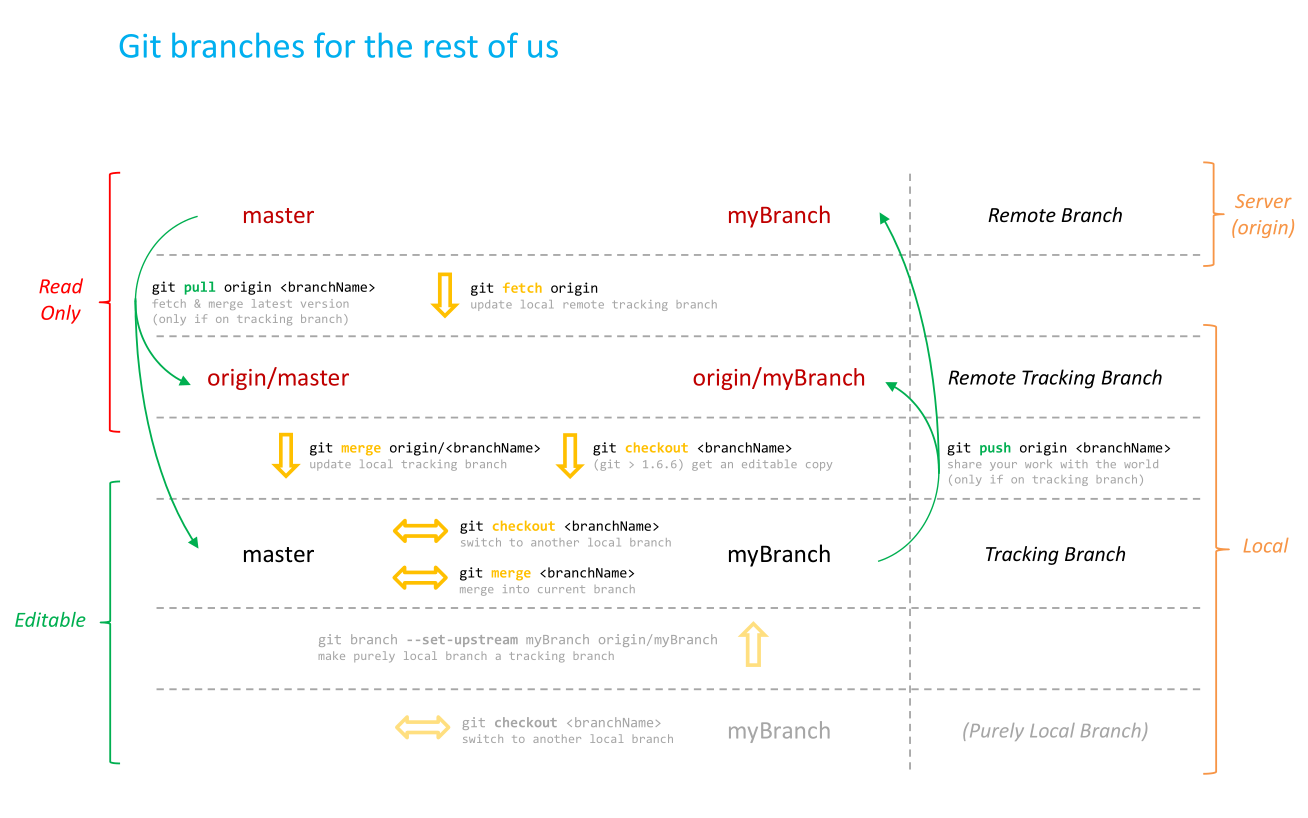
\includegraphics[width=6.26806in,height=3.92014in,alt={A picture containing table Description automatically generated}]{assets/media/image12.png}
\end{center}

Na slikama ispod je prikazana razmjena izmjena. Miloš je napravio neke
izmjene koje šalje na udaljeni repozitorijum. Kad su izmjene poslate na
udaljeni repozitorijum, Marko može da ih preuzme u svoju lokalnu kopiju
main-a i nastavi sa razvojem.

\begin{center}
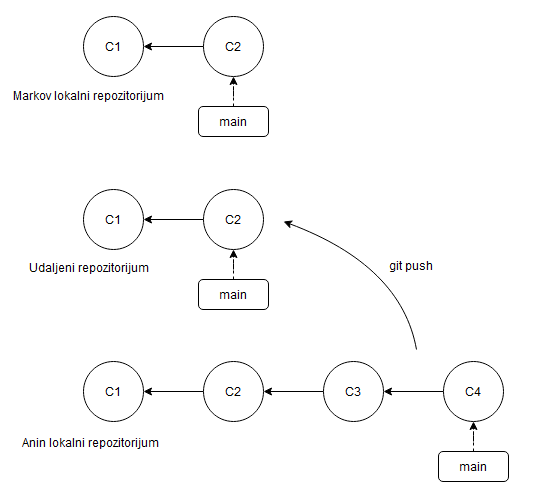
\includegraphics[width=2.03188in,height=1.81102in,alt={Diagram, schematic Description automatically generated}]{assets/media/image13.png}
\end{center}
\begin{center}
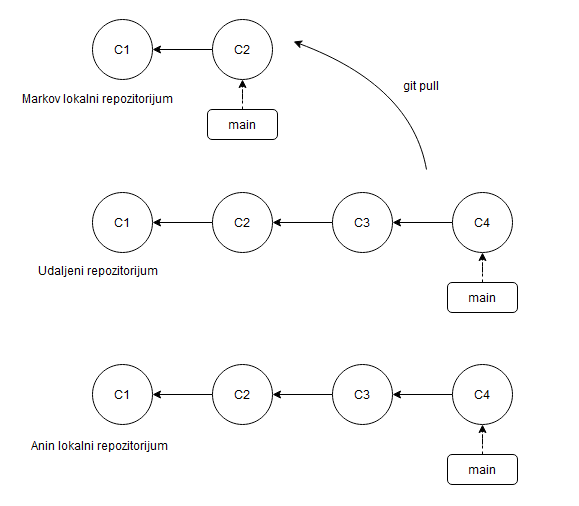
\includegraphics[width=2.0723in,height=1.81102in,alt={Diagram Description automatically generated}]{assets/media/image14.png}
\end{center}
\begin{center}
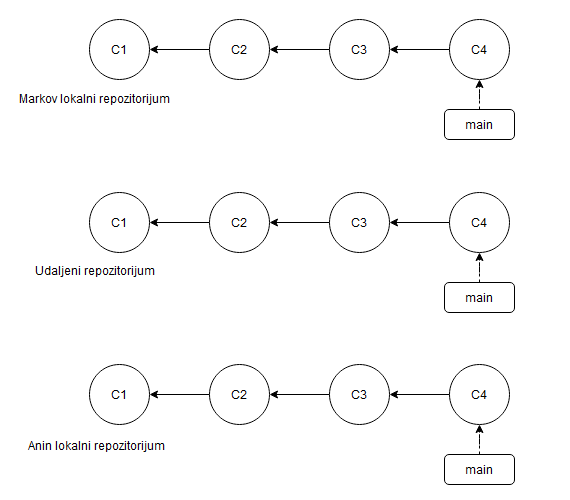
\includegraphics[width=2.06457in,height=1.81102in,alt={Diagram Description automatically generated}]{assets/media/image15.png}
\end{center}

\subsection{Kloniranje udaljenog
repozitorijuma}

Postavlja se pitanje kako možemo da preuzmemo stanje udaljenog
repozitorijuma kojeg nemamo lokalno na računaru. To radimo sa naredbom
\emph{clone} na idući način: git clone \textless url do udaljenog
repozitorijuma\textgreater. Sa ovim će git preuzeti udaljeni
repozitorijum, napraviti novi folder sa njegovim imenom i u njega će
smjestiti sve fajlove i sve izmjene zabilježene u istoriji tog udaljenog
repozitorijuma. Nakon clone-a možemo nastaviti rad na repozitorijumu.
Isprobaj ovu naredbu tako što ćeš klonirati idući repozitorijum:
\url{https://github.com/SIIT-USI/git-clone-test}.

\section{Vježbanje rada sa
granama}

Da bi izvježbao rad sa granama, kako lokalnim, tako i remote, pređi
vježbe sa ovog sajta \url{https://learngitbranching.js.org/} vezane za
rad sa granama.

\section{Pull request}

Pull request (PR) je proces putem kog se novi kod integriše na udaljeni
repozitorijum. Ideja iza PR je da se kod prije spajanja sa
repozitorijumom provjeri za greške, iztestira kako bi se povećao
kvalitet koda i projekta. PR je kao neka kontrola merge naredbe, gdje
neku granu umjesto da spojiš lokalno, napraviš PR pomoću kog ćeš je
spojiti. Tako se prije spajanja lako može provjeriti kod za greške.
Spajanjem PR-a se i same grane razvoja spoje.

PR možeš napraviti putem GitHub-a. Otvori Pull request tab
repozitorijuma u kojem želiš da otvoriš PR i pritisnite na ``New pull
request''.

\begin{center}
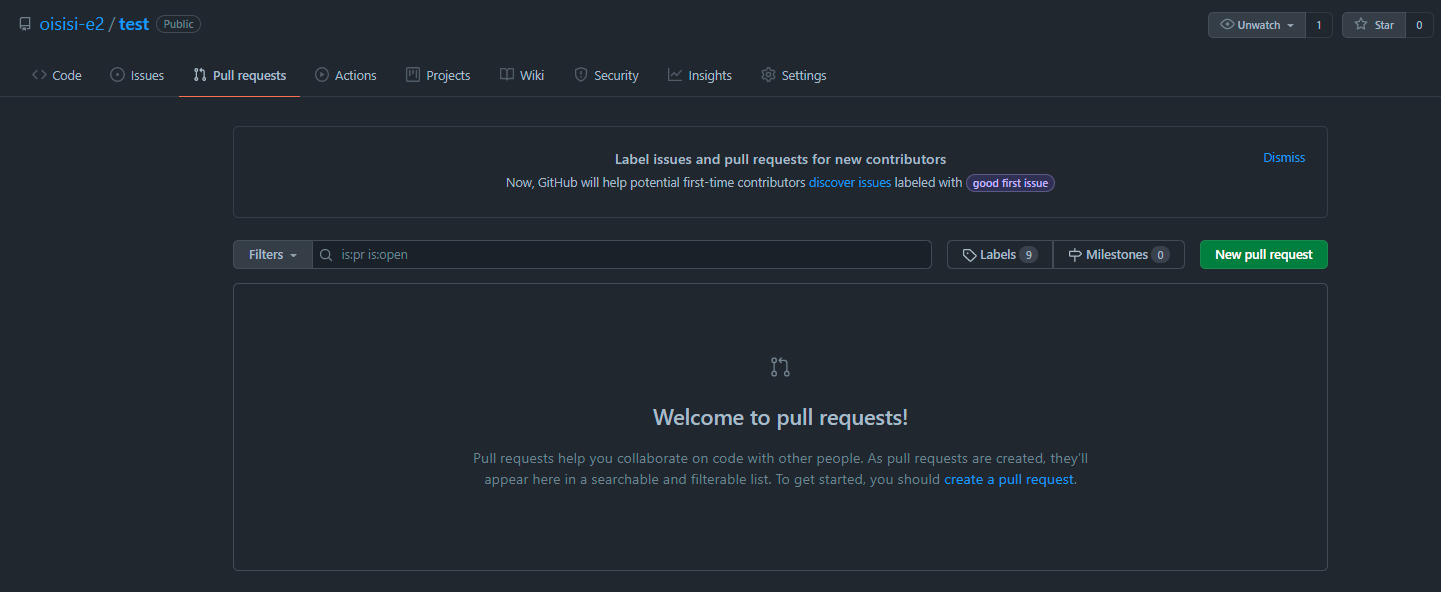
\includegraphics[width=6.05628in,height=2.488in,alt={A screenshot of a computer Description automatically generated with medium confidence}]{assets/media/image16.png}
\end{center}

Idući korak je prikazan na slici ispod. Potrebno je da odabereš koju
granu želiš da spojiš na koju granu. Ispod možeš da pogledaš pregled
commit-ova i pregled izmjena.

\begin{center}
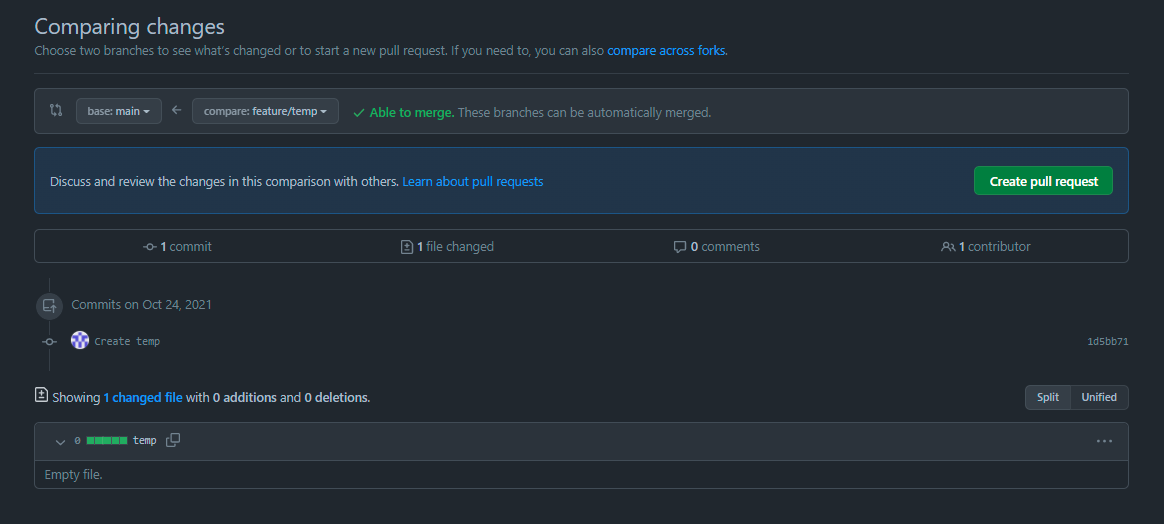
\includegraphics[width=5.97142in,height=2.688in,alt={A screenshot of a computer Description automatically generated}]{assets/media/image17.png}
\end{center}

Nakon pritiska na dugme ``Create pull request'' otvori se prozor sa
slike ispod. Tu možemo da podesimo naziv PR-a kao i opis -- šta smo
izmijenili i zašto. Dalje, moguće je podesiti ``Reviewers'' grupu ljudi
koji treba da odrade review novih izmjene. ``Assignees'' grupa ljudi
koja je zadužena za PR -- ljudi koju su pravili izmjene. Obično je to
osoba koja pravi PR. ``Labels'' su kao tagovi sa kojima možeš da označiš
PR, pa kasnije koristiš za filtriranje.

Kad sve popuniš, pritisni na ``Create pull request'' da bi napravio PR.

\begin{center}
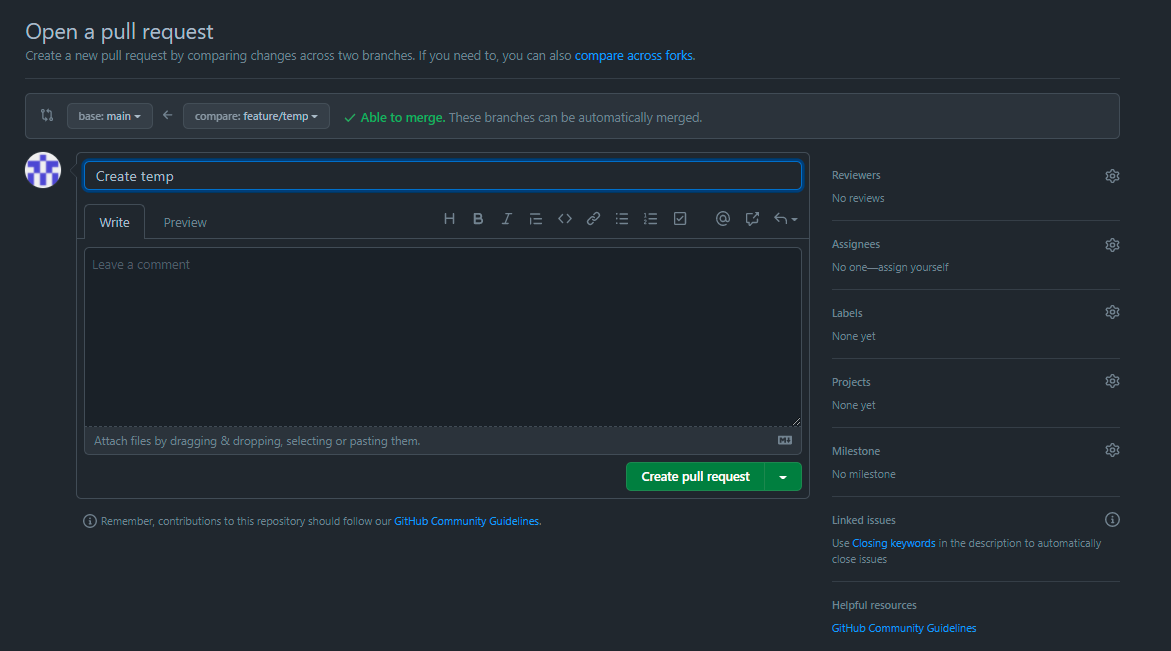
\includegraphics[width=6.01494in,height=3.344in,alt={A screenshot of a computer Description automatically generated}]{assets/media/image18.png}
\end{center}

Otvoren PR je prikazan na slici ispod.

\begin{center}
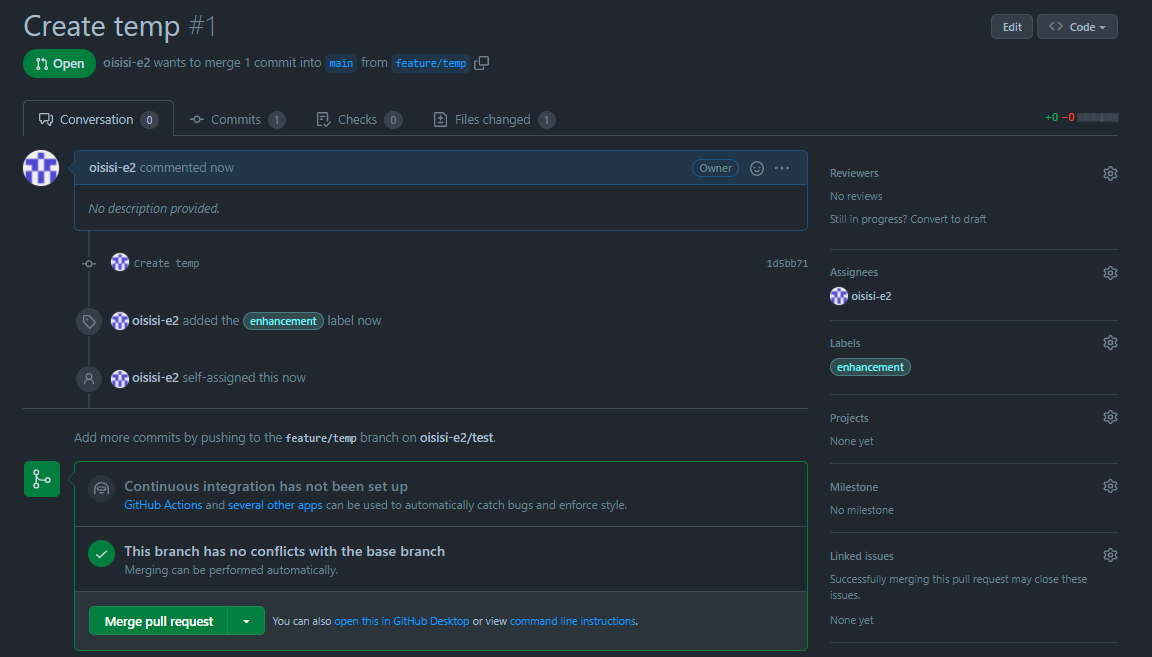
\includegraphics[width=4.608in,height=2.62818in,alt={A screenshot of a computer Description automatically generated with medium confidence}]{assets/media/image19.png}
\end{center}

Pod tabom ``Files changed'' možeš da odradiš review PR-a. Review
podrazumijeva da prođeš kroz sve izmjene, testiraš sve, uvjeriš se da
radi kako je zamišljeno. Usput ostavljaj komentare na mjestima koje
treba izmijeniti ili ako želiš da prodiskutuješ o načinu implementacije
sa kolegom koji je napravio PR, i slično. Na dugme „Review changes``
kreiraš review. Možeš da:

\begin{itemize}
\item
  odobriš izmjene i dozvoliš kolegi da spoji izmjene u granu u koju želi
\item
  samo ostaviš komentar bez eksplicitnog odobrenja ili
\item
  možeš da zatražiš izmjene i onemogućiš spajanje dok se ne dodaju
  tražene izmjene.
\end{itemize}

\begin{center}
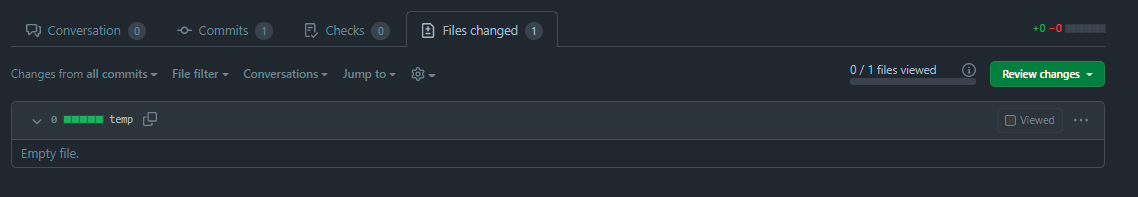
\includegraphics[width=6.26806in,height=1.08472in,alt={Graphical user interface, application Description automatically generated}]{assets/media/image20.png}
\end{center}

Kad dobiješ sve dozvole za merge od svih review-era možeš da odradiš
merge i spojiš svoje izmjene. Spojen PR je prikazan ispod

\begin{center}
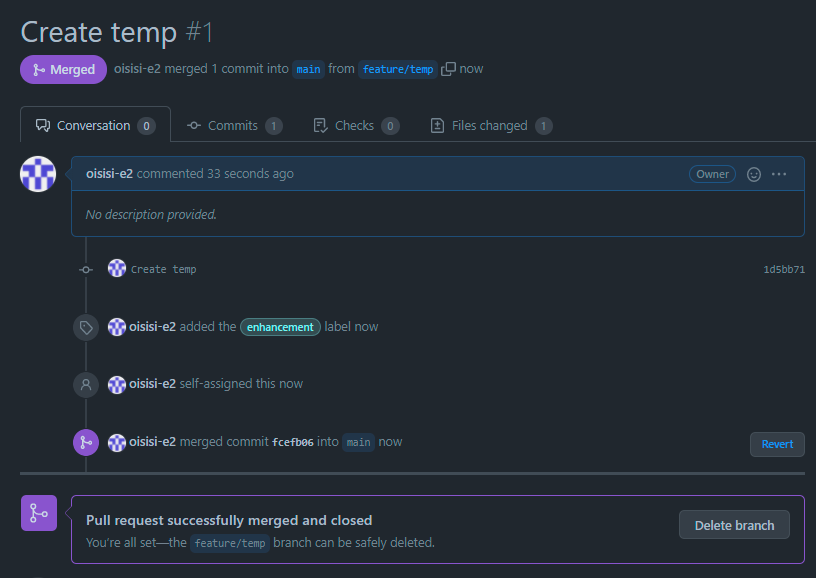
\includegraphics[width=4.392in,height=3.11128in,alt={A screenshot of a computer Description automatically generated}]{assets/media/image21.png}
\end{center}

\section{Dodatna konfiguracija}

Prilikom svakog push-a na udaljeni repozitorijum git će tražiti da
unesete kredencijale za pristup. Ovo možete izbjeći tako što podesiš
SSL. GitHub ima
\href{https://docs.github.com/en/authentication/connecting-to-github-with-ssh}{tutorial},
za GitLab su slični koraci, jedina razlika je u dodavanju SSH ključa u
vaš profil na GitLab.

Kako bi ubrzali rad sa gitom preporučujem da napravite git aliase. Alias
je skraćeno ime za pisanje čestih git komandi. Pogledajte
\href{https://git-scm.com/book/en/v2/Git-Basics-Git-Aliases}{dokumentaciju}
za detalje i primjere.

\section{Literatura i inspiracija}

\begin{itemize}
\item
  \url{https://git-scm.com/book/en/v2} - Pro git knjiga (git Biblija),
  preporučuje se da pročitaš prva 3 poglavlja
\item
  \url{https://missing.csail.mit.edu/2020/version-control/} - video i
  tekstualni materijali MIT-a o git-u
\item
  \url{http://www.igordejanovic.net/courses/tech/git/} - odlični
  slajdovi koje je napravio profesor Dejanović, osnovni i napredni
  pojmovi su detaljno objašnjeni. Dodatno, sve je na srpskom.
\end{itemize}

\end{document}
